\documentclass{article}

\usepackage[top=2cm, bottom=2cm]{geometry}
\usepackage[utf8]{inputenc} % allow utf-8 input
\usepackage[T1]{fontenc}    % use 8-bit T1 fonts
\usepackage{hyperref}       % hyperlinks
\usepackage{url}            % simple URL typesetting
\usepackage{booktabs}       % professional-quality tables
\usepackage{microtype}      % microtypography
\usepackage{graphicx}
%\usepackage{subfigure}
\usepackage{subcaption}
\usepackage{hyperref}       % hyperlinks
\usepackage{tikz}           % define for loops

\hypersetup{ % SLJ: my standard paper setup...
	pdftitle={MAP convergence},
	pdfkeywords={},
	pdfborder=0 0 0,
	pdfpagemode=UseNone,
	colorlinks=true,
	linkcolor=blue, %mydarkblue,
	citecolor=blue, %mydarkblue,
	filecolor=blue, %mydarkblue,
	urlcolor=blue, %mydarkblue,
	pdfview=FitH,
	pdfauthor={Anonymous},
}

\usepackage[round]{natbib}
\renewcommand{\bibname}{References}
\renewcommand{\bibsection}{\subsection*{\bibname}}

\newcommand{\RLP}[1]{\textcolor{red}{RLP:#1}}
\newcommand{\violet}[1]{\textcolor{violet}{#1}}
\newcommand{\TODO}[1]{\textcolor{cyan}{TODO #1}}

% my packages
\usepackage{math_commands}
% some custom math commands
\newtheorem{proposition}{Proposition}
\newcommand*{\expect}[2][]{\ensuremath{\mathbb{E}_{#1} \left[ #2 \right] }} % expectation operator
\newcommand{\logpart}{A}
\newcommand{\conj}{\logpart^*}
\newcommand{\bregman}{\cB_\logpart}
\newcommand{\bregmanconj}{\cB_{\logpart^*}}
\newcommand{\natp}{\theta}
\newcommand{\meanp}{\mu}
\newcommand{\decrement}{D}
\newcommand{\Dir}{\mathrm{Dir}} % Dirichlet
\newcommand{\linear}{\ell} % linearization of a function
\newcommand{\lr}{\gamma} % learning rate, or step-size


\title{Convergence rate of MAP estimates \\
for the exponential family}
\author{R\'emi Le Priol}
\date{October 2020}


\begin{document}

\maketitle

\section{Background}

\paragraph{Motivation.} 
We do not know general convergence rates on the KL for maximum likelihood estimates of the exponential family.  We want the simplest one.
We hope  to get a new result by combining tools from statistics and optimization. 

\paragraph{Exponential Family.}
The exponential family member with sufficient statistic $T$ and natural parameter $\natp$ is the model
\begin{align}
    p(X|\natp) &= \exp( \natp^\top T(X) - \logpart(\natp)) \; ,
\end{align}
with log-partition function 
\begin{align}
    \logpart(\natp) = \log \int e^{\natp^\top T(x)} dx \; .
\end{align}
Recall that $\logpart$ verifies the two following identities 
\begin{align}
    \nabla\logpart(\natp) &=  \expect[p(X|\natp)]{T(X)} =: \meanp \\
    \nabla^2 \logpart(\natp) &= \Cov_\natp[T(X)] > 0
\end{align}
where $\meanp$ is called the mean parameter.
The second identity entails that $\logpart$ is strictly-convex.

\paragraph{Conjugate Prior}
The conjugate prior for $p(X|\natp)$ is
\begin{align}
    \pi(\natp) &\propto \exp( - n_0 \bregman(\natp ; \natp_0) )
\end{align}
where $n_0$ and $\natp_0$ are (hyper)parameters of the prior.
Intuitively, $n_0$ is a number of fictive points observed from a distribution with parameter $\natp_0$.
Finally, $\bregman(\natp ; \natp_0)$ is the Bregman divergence induced by $\logpart$ between $\natp$ and $\natp_0$
\begin{align}
    \bregman (\natp ; \natp_0)
    & = \logpart(\natp) - \logpart(\natp_0) 
    - \langle \nabla \logpart(\natp_0)  , \natp - \natp_0 \rangle
\end{align}
with $\nabla \logpart(\natp_0) = \expect[\natp_0]{T(X)} =: \meanp_0$ the mean parameter associated to $\natp_0$.

\paragraph{MAP.}
The negative log-likelihood of the prior is then
\begin{align*}
    -\log \pi(\natp) = n_0 (\logpart(\natp)  - \natp^\top \meanp_0 ) + \cst
\end{align*}
Thus the joint NLL of $(x_1,\dots,x_n,\natp)$ is
\begin{align}
    -\log p(X|\natp)\pi(\natp) 
    = (n_0+n) \logpart (\natp) 
    - \theta^\top \left(n_0 \meanp_0 + \sum_{i=1}^n T(x_i) \right) + \cst \; .
\end{align}
Minimizing this expression over $\natp$ yields the Maximum A Posteriori estimate
\begin{align}
    \hat \natp = \argmin_\natp -\log p(X|\natp) + n_0 \bregman(\natp ; \natp_0)
\end{align}
such that the MAP is
\begin{align}
    \nabla \logpart(\hat \natp) = \hat \meanp
    = \frac{n_0 \meanp_0 + \sum_{i=1}^n T(X_i) }{n_0+n} \; .
\end{align}
The MAP estimate is a random quantity. We wish to bound its deviation the optimum $\natp^*$ or $\meanp^*$.


\section{Straightforward Convergence Rate}
In the realizable case, the suboptimality on the population log-likelihood is exactly the KL between our current model and the true distribution
\begin{align}
    &\expect[X\sim p(.|\natp^*)]{-\log p(X|\natp) + \log p(X|\natp^*)}\\
    =& \KL( p(.|\natp^*) ; p(.|\natp)) \\
    =& \bregman (\natp ; \natp^*) \\
    =& \bregmanconj ( \meanp^* ; \meanp) \\
    =& \conj(\mu^*) + \logpart(\natp) - \langle \natp , \mu^* \rangle
    %& = \logpart(\natp) - \logpart(\natp^*) - \meanp^{*\top}(\natp - \natp^*) \; .
\end{align}
where $\conj$ is the entropy, the convex conjugate of the log-partition.
The relationship between Bregman divergences and Fenchel conjugacy is well explained in \citet{wainwright2008graphical}, and \citet{agarwal2010geometric}. 
The question is: how does this quantity behave when $\natp$ is the maximum-likelihood or the MAP estimate ? Can we get bounds -- in expectation or high-probability -- on the following quantities ?
\begin{align}
	\label{eq:bregmanMLE}
	\bregmanconj \left (\E [T(X)] ;  \inv{n}  \smallsum_i T(X_i) \right ) \; , \\
	\label{eq:bregmanMAP}
	\bregmanconj \left (\E [T(X)] ; \frac{n_0 \mu_0 + \smallsum_i T(X_i)}{n_0+n} \right ) \; .
\end{align}

\paragraph{If $\conj$ is $L$-Lipschitz} (e.g. $\logpart$ is defined within the $\ell^2$-ball of radius $L$), then
\begin{align}
    \bregmanconj(\mu^* ; \mu) 
    \leq L \norm{\mu^* - \mu} + \norm{\natp} \norm{\mu^* - \mu}
    \leq 2L \norm{\mu^* - \mu}
\end{align}
so $\bregmanconj$ is $2L$-Lipschitz.
Since the empirical average converges in expectation to the population mean at a rate of $1/\sqrt{n}$ in $\ell^2$ norm, we know that this bound applies to the log-likelihood.

\paragraph{If $\conj$ is $L$-smooth} (e.g. $\logpart$ is $L^{-1}$-strongly convex), then
\begin{align}
    \bregmanconj(\mu^* ; \mu) 
    \leq \frac{L}{2} \norm{\mu^* - \mu}^2
\end{align}
so $\bregmanconj$ is upper bounded by a quadratic. In expectation, it should converge at a rate $1/n$.

\paragraph{$\ell^2$-norm analysis}
Let us make these statements more precise. A bound on the variance becomes a bound on the variance of the average
\begin{align}
	\Var T(X) = \E \norm{T(X) - \mu^*}^2 = \sigma^2 \\
	\implies \E \norm{\mu^* -  \inv{n}  \smallsum_i T(x_i)}^2 = \frac{\sigma^2}{n} 
\end{align}
eg the variance of the mean is $n$ times smaller than the variance of the samples.
Adding a reference mean $\mu_0$ to get the MAP yields
\begin{align}
	\E \norm{\mu^* -  \frac{n_0 \mu_0 + \smallsum_i T(x_i)}{n_0+n} }^2 
	&= \frac{n}{(n+n_0)^2} \sigma^2 +  \frac{n_0^2}{(n+n_0)^2} \norm{\mu^* -  \mu_0}^2 \\
	&= O\left(\frac{\sigma^2}{n} \right) + O\left(\frac{\norm{\mu^* -  \mu_0}^2}{n^2} \right)
\end{align}
so we have a variance term in $O(n^{-1})$ and a bias term decreasing as $O(n^{-2})$. Let's see if we can get similar estimates for arbitrary exponential families !

In the limit, the MAP estimates reach a rate $O(1/2n)$. This is shown by approximating the Bregman divergence using a second order Taylor expansion
\begin{align}
    \bregmanconj(\mu^* ; \mu) 
    &= \half (\mu - \mu^*)^\top \nabla^2\conj(\mu^*)(\mu - \mu^*)  
    + O(\norm{\mu - \mu^*}^3)\\
    &=\half  \norm{\mu^* - \mu}^2_{\nabla^2\conj(\mu^*)}
    + O(\norm{\mu - \mu^*}^3)
\end{align}
where we introduced the Mahalanobis distance induced by the matrix 
\begin{align}
    \nabla^2\conj(\mu^*) 
    = \nabla^2\logpart(\natp^*)^{-1} 
    = \Cov_{\natp^*}[T(X)]^{-1} 
    =: \mSigma^{-1}  \; .
\end{align}
To exploit this approximation, let us extend the $\ell^2$ norm results to a Mahalanobis distance induced by matrix $\mM$
\begin{align}
	\E \norm{\mu^* -  \inv{n}  \smallsum_i T(x_i)}_\mM^2 = \inv{n} \Tr(\mM \mSigma)
\end{align}
where $\mSigma$ is the covariance of $T(X)$. We retrieve $\nicefrac{\sigma^2}{n}$, the variance divided by the number of samples, when the metric is the identity $\mM=\mI$.  For the MLE we get
\begin{align}
	\E \bregmanconj \left (\E [T(X)] ;  \inv{n}  \smallsum_i T(X_i) \right ) = \frac{d}{2n} + O(n^{- \frac{3}{2}})
\end{align}
and for the MAP we  get 
\begin{align}
	\E \norm{\mu^* -  \frac{n_0 \mu_0 + \smallsum_i T(x_i)}{n_0+n} }^2_{\mSigma^{-1}}
	&= \frac{n d}{(n+n_0)^2}  +  \frac{n_0^2}{(n+n_0)^2} \norm{\mu^* -  \mu_0}^2_{\mSigma^{-1}} \\
	&= O\left(\frac{d}{n} \right) + O\left(\frac{\norm{\mu^* -  \mu_0}^2_{\mSigma^{-1}} }{n^2} \right) \; .
\end{align}
Remark how the variance does not even appear, only the dimension divided by $n$ really matters. I find this result quite spectacular : the convergence speed of MLE is not affected by the covariance of sufficient statistics, and for MAP it matters only in the $O(n^{-2})$ term.
Indeed this is because it is hidden within the Bregman divergence loss. 
Anyway that's all good for asymptotic results, but we are interested in a finite sample analysis. How do we get this ?

\subsection{Cramer-Rao Lower Bound}
In statistics, there is this famous theorem known as the Cramer-Rao lower bound. In its simplest form, it states that the covariance of an unbiased estimator of a distribution's parameter $\natp$ is lower bounded by the inverse Fisher information matrix, divided by $n$
\begin{align}
    \Cov(\hat \natp_n)  
    &\succeq \inv{n} \cI(\natp_*)^{-1} \\
    \iff
    \expect[\cD\sim \natp_*]{(\hat \natp_n - \natp_*)(\hat \natp_n - \natp_*)^T}
    &\succeq \inv{n} \expect[X\sim \natp_*]{-\nabla^2 \log p(X|\natp_*)}^{-1} \; .
\end{align}
This is a typical statistic bound, which is concerned with the $\ell^2$ accuracy of an estimator, via its covariance. In contrast, here we are concerned with the quality of the estimator in terms of KL-divergence, eg "how accurately am I modeling this distribution?"

Note that in the case of an exponential family, the lower bound is always reached for the MLE estimator $\hat \mu_n$, because $\cI(\mu) = \nabla^2 \conj(\mu) = \nabla^2 \logpart(\natp)^{-1} = \Cov(T(X))^{-1}$, where the first step takes some calculus. For the estimator $\hat \natp_n$, this lower bound is not trivial.

\subsection{Posterior Expected Loss}

A conjugate prior for the exponential family with sufficient statistic $T(X)$ and natural parameter $\natp$ is 
\begin{align}
    \pi(\natp) 
    \propto \exp(-n_0 \bregman(\natp ; \natp_0)) 
    \propto \exp(-n_0 \logpart(\natp) + \langle n_0 \mu_0 ; \natp \rangle)
\end{align}
so we see that $\pi$ is part of the exponential family, with sufficient statistic $(\natp, \logpart(\natp))$ and natural parameters $(n_0 \mu_0 , -n_0)$. When we update this prior with Bayes formula on dataset $\cD=(x_1,\dots,x_n)$, we get a posterior $\pi(\natp | \cD)$ with natural parameters $(n_0 \mu_0 + \sum_i T(x_i) , -(n_0 + n))$. This is well detailed in \citet{agarwal2010geometric}. 

Given this posterior, a natural quantity to consider is the expected loss. Thus we might ask "what is the expectation of the posterior expected suboptimality?"
\begin{align}
    \expect[\cD\sim\natp_*]{\expect[\pi(\natp|\cD)]{\bregman(\natp ; \natp_*)}}
\end{align}
This quantity is even harder to estimate than the expected MAP suboptimality, because of the double integral. We can get a closed form for the age-old $\ell^2$ loss of $\cN(\mu, 1)$, which yields the exact rate $\inv{n}$. This is exactly twice the expected loss of the MAP.

\section{Stochastic Bregman Proximal Point}
We see that the MAP estimate minimizes the sum of a stochastic loss $ -\log p(X|\natp)$ and a deterministic divergence to an initial point $n_0 \bregman(\natp ; \natp_0)$. This is a stochastic Bregman proximal step with step-size $\inv{n_0}$. This can also be seen at each step since
\begin{align}
    \hat \natp_{n+1} 
    &= \argmin_\natp -\log p(x_{n}|\natp) + (n_0 + n) \bregman(\natp ; \hat \natp_n) \\
    &= \argmin_\natp f(\natp; x_{n}) +  \inv{\gamma_{n}}\bregman(\natp ; \hat \natp_n) \; .
\end{align}
Hence the MAP estimate can also be seen as the result of a stochastic proximal Bregman point algorithm with step-size $\gamma_n = \inv{n_0 + n}$ at step $n$.

This is similar to the online learning setup, and it may be possible to bound the regret, with approaches similar to Adagrad.

The analysis of deterministic Bregman proximal point relies on the three points lemma (Appendix~\ref{app:3points}). First one can prove descent, then one can prove that the total path length and the sum of suboptimalities are bounded, but this does not transpose immediately to the stochastic setting. One needs an assumption on the quality of the stochastic estimates $f(. ; x)$. 
\RLP{Write down the formulas going with this text.}
Given the proof, the most straightforward such assumption is 
\begin{align}
\expect{f(\natp_{n+1}) - f(\natp_{n+1} ; x_{n})} \leq \gamma_n \sigma^2
\end{align}
which translates to $\Cov(T(x_{n}) , \natp_{n+1}) \leq  \gamma_n \sigma^2$ in our case. This is exactly the same assumption as given by the SMD analysis. However even with this assumption, the convergence rate applies to the iterate $\sum_t \lr_t \natp_{t+1} / \sum_t \lr_t$, which gives more weight to the first iterates. It does not immediately apply to the last iterate.


\section{Stochastic Mirror Descent (SMD)}
\subsection{MAP as SMD}
Let $f(\natp) := \expect[x]{-\log p(x|\natp)} = - \langle \mu_*, \natp\rangle + \logpart(\natp)$. In words, $f$ is linear modification of a convex function $\logpart$, which we can access only through noisy estimates of $\mu_*$. It turns out that the MAP estimate can also be seen as the iterates of stochastic mirror descent with mirror map $\logpart$. First let's recall mirror descent iteration
\begin{align}
	\natp_{t+1} 
	&:= \argmin_\natp \lr \linear_f(\natp; \natp_t) + \bregman(\natp ; \natp_t)  \\
	& = \nabla \conj (\nabla \logpart(\natp_t) - \lr \nabla f(\natp_t))
\end{align}
where $\linear_f(\natp; \natp_t) = f(\natp_t) + \langle \nabla f(\natp_t), \natp - \natp_t \rangle$ is the linear approximation of $f$ in $\natp_t$ evaluated at $\natp$. Solving this problem require solving problems of the form $\argmin_\natp - \langle c, \natp \rangle + \logpart(\natp)$, eg computing the convex conjugate of $\logpart$. 
Note that finding $\natp_*$ is done with 1 step of mirror descent. Indeed plugging in definitions of $f$ and $\mu$ yields
\begin{align}
	&\mu_{t+1}  = \mu_t - \lr (\mu_t - \mu_*) \\
	\implies &\mu_t  = \mu_* + (1- \lr)^t (\mu_0 - \mu_*)
\end{align}
which shows exponential convergence and 1-step convergence when $\lr =1$. Back to our sheep, the MAP iteration can be cast as stochastic mirror descent (SMD),  with $g_t = \nabla f(\natp_t, x_{t+1})$ a stochastic estimate  of $\nabla f(\natp_t)$
\begin{align}
    \hat \natp_{n+1} 
    &= \argmin_\natp 
    - \langle T(x_{t+1}), \natp \rangle  + \logpart(\natp) + (n_0 + n) \bregman(\natp ; \natp_n) \\
    %&(n_0+n)\left(\logpart(\natp) - \logpart(\natp_n) - \langle \nabla \logpart(\natp_n)  , \natp - \natp_n \rangle \right)  \\
    &= \argmin_\natp - \langle T(x_{t+1}), \natp \rangle   + \logpart(\natp_n) + \langle \nabla \logpart(\natp_n)  , \natp - \natp_n \rangle + (n_0+n + 1) \bregman(\natp ; \natp_n) \\
    &= \argmin_\natp \linear_f(\natp;\natp_n, x_{t+1}) + (n_0 + n + 1) \bregman(\natp ; \natp_n)
\end{align}
where $\linear_f(\natp;\natp_n, x_{t+1})$ is the stochastic linearization of $f$ at $\natp_n$ evaluated at $\natp$ with randomness coming from $x_{t+1}$. This is the formula for stochastic mirror descent (SMD) applied to $f$ with mirror map $\logpart$ and step-size $\gamma_n = \inv{n_0 + n + 1}$.

\subsection{Relative Smoothness for Mirror Descent}
In the classic setting, SMD is studied under strong-convexity assumption on the mirror map $\logpart$ \citep{bubeck2015convex}.
In our setting this is not always true -- eg gaussians.
However a recent and fast-expanding body of work is concerned with a new assumption: relative smoothness and relative strong-convexity.
\begin{align}
	& \text{$f$ is $L$-smooth relative to $h$} \\
	\iff & Lh - f \ \text{convex} \\
	\iff & f(y) \leq 	f(x) + \langle \nabla f(x) , y-x \rangle + L\cB_h(y;x), \forall x,y \\
	\iff & \cB_f(y;x) \leq L \cB_h(y;x), \forall x,y \\
	\iff & \nabla^2 f(x) \leq L \nabla^2 h(x),  \forall x
\end{align} 
where the last equivalence holds only when $f$ and $h$ are twice differentiable. In words, $f$ is upper bounded by it linear approximation plus the $h$-Bregman divergence, which can also be seen as a bound between divergences, or more locally as a bound between Hessians. Similarly, $f$ is $\mu$ strongly-convex relative to $h$ if
\begin{align}
	& f-\mu h \ \text{ convex} \\
	\iff & f(x) + \langle \nabla f(x) , y-x \rangle + \mu \cB_h(y;x) \leq f(y)\forall x,y \\
	\iff & \mu\cB_h(y;x) \leq \cB_f(y;x) \forall x,y \\
	\iff & \mu \nabla^2 h(x) \leq \nabla^2 f(x)  \forall x \; .
\end{align} 

Another way to view this elegant generalization of smoothness and strong-convexity is as a transfer of the Loewner partial order on symmetric matrices to functions, via the Hessian. 
As such it can be applied to many functions that were out of reach for $\ell^2$ norm, by taking the appropriate reference function.  For instance $h(x) = -\log(x)$ or $h(x) = x^4$. 
As early as 2011, \citet{birnbaum2011distributed} showed $O(\inv{t})$ convergence rate for mirror descent under smoothness assumption relative to the mirror map. 
More precisely, he proved that when $f$ is $L$-smooth relative to $h$, then the suboptimality of the sequence 
\begin{align}
	x_{t+1}  = \argmin_x \langle \nabla f(x_t), x \rangle + \cB_h(x ; x_t)
\end{align}
is upper bounded by the simple formula
\begin{align}
	\implies f(x_t) - f(x_*) \leq \frac{L \cB_h(x_* ; x_0) }{t} \; .
\end{align}
These notions were rediscovered and expanded by \citet{bauschke2017descent} and \citet{lu2018relatively}. If you need to read one, pick \citet{lu2018relatively} -- I found it much much easier and more enjoyable to read.  This latter paper also derived a linear convergence rate for mirror descent under relative smoothness and strong-convexity, with the relative condition number $\frac{L}{\mu}$ appearing.

\subsection{Relative smoothness for SMD}
Now our setting is Stochastic Mirror Descent (SMD), meaning at each step we observe a random unbiased estimate gradient. This setting was studied by \citet{hanzely2018fastest}, who proved in the smooth strongly-convex case with tail averaging :  with constant step-size, linear convergence down to a variance ball, and with step-size $\gamma_t = n_0 + t$ a rate $\tilde O(\inv{t})$. These results match the rates for standard SGD.

This is very interesting for us, but the variance hyper-parameter is oddly defined. Let $g_t$ be the random gradient at step $t$  (coming from data point $x_t$), and $\natp_{t+1}$ the next iterate. Then the variance bound $\sigma^2$ is an upper bound on the covariance between the gradient update  $-g_t$ and the descent direction $\natp_{t+1} - \natp_t = \nabla \logpart^*(\nabla \logpart(\natp_t) - \lr_t g_t ) - \natp_t $ that should hold for all time steps  
\begin{align}
	&\Cov(- g_t,\natp_{t+1} - \natp_t | X_{1 \dots t}) \leq \lr_t \sigma^2 \\
	&= \expect{\langle - g_t, \natp_{t+1} \rangle}  - \langle \E[-g_t], \E[\natp_{t+1}] \rangle   \\
	 &= \expect{\langle \nabla f(\natp_t) - g_t , \natp_{t+1}  \rangle}
\end{align}
where $\gamma_t$ is the step-size and expectations are conditional on the past. Remark that when we plug in $\conj = \|.\|^2$, we recover the gradient variance typical of SGD. In our case, 
\begin{align}
	\nabla f(\natp_t) - g_t =  T(X_{t+1})	- \E[T(X)]
\end{align}
so that $\sigma$ is really a bound on the covariance of the sufficient statistics with another variable
\begin{align}
	&\Cov( T(X_{t+1}), \natp_{t+1}| X_{1\dots t})
	\leq \lr_t\sigma^2 \\
	=& \Cov(T(X_{t+1}), \nabla\conj \left(\lr_t T(X_{t+1}) + (1-\lr_t ) \mu_t \right) | X_{1\dots t}) \;.
\end{align}
In other words, we need for all $\lr\in(0,\inv{n})$, and $ \mu$ in the interior of the marginal polytope,
\begin{align}
\label{eq:hypvariance}
	\Cov_X \bigg(T(X), \nabla \conj (\lr T(X) + (1-\lr) \mu)\bigg	) 
	\leq \lr \sigma^2 \; .
\end{align}
We study this assumption in Section \ref{sec:gaussian_variance} where we show that it cannot hold in general for the $\mu$ we care about. 
When we plug this bound into the expected suboptimality formula~\eqref{eq:bregmanMLE} with the maximum likelihood estimate $\hat \mu =  \inv{n}\sum_i T(X_i)$, assuming all $T(x)$ belong to the marginal polytope, we get
\begin{multline}
	\expect[X_{1\dots n}]{\bregmanconj ( \mu_* ;\hat \mu) }
	=\conj(\mu_*) \overbrace{- \E[\conj(\hat \mu)]}^{\leq - \conj(\E[\hat \mu])} \\
	+ \inv{n}\sum_i \E[\underbrace{\E[\langle  T(X_i) - \mu_*; \nabla\conj (\hat \mu) \rangle | X_j, j\neq i]}_{\leq \nicefrac{\sigma^2}{n} \eqref{eq:hypvariance}
	 	\; \text{with}\; \mu=\inv{n-1}\smallsum_{j\neq i} T(x_j)  } ]  \leq \frac{\sigma^2}{n}
\end{multline}
\textcolor{red}{what about:}
\begin{multline}
	\expect[X_{1\dots n}]{\bregmanconj ( \mu_* ;\hat \mu) }
	=\conj(\mu_*) \overbrace{- \E[\conj(\hat \mu)]}^{\leq - \conj(\E[\hat \mu])} \\
	+ \inv{n}\sum_i \E[\underbrace{\E[\langle  T(X_i) \textcolor{red}{- \hat \mu_{n-1} + \hat \mu_{n-1}} - \mu_*; \nabla\conj (\hat \mu) \rangle | X_j, j\neq i]}_{\leq \nicefrac{\sigma^2}{n} \eqref{eq:hypvariance} } ]  \leq \frac{\sigma^2}{n}
\end{multline}
where we used the decomposition $\hat \mu = \inv{n}T(X_i) + (1-\inv{n}) \inv{n-1} \sum_{j\neq i}T(X_j)$ to apply~\eqref{eq:hypvariance}. 
In words, this variance assumption on $T(X)$ and $\conj$ immediately gives us a bound on the suboptimality. We can also apply this result to the MAP estimate $\hat \mu = \frac{n_0 \mu_0 + \smallsum_i T(X_i)}{n_0+n}$ but I did not manage to reach a satisfying conclusion about the bias. 
Note $\tilde \mu = \E[\hat \mu] = \frac{n_0 \mu_0 + n \mu_*}{n_0+n}$ and $\gamma_0= \frac{n_0}{n_0+n}$ and the step-size $\gamma = \inv{n_0 + n}$ .
\begin{align}
	\expect[X_{1\dots n}]{\bregmanconj ( \mu_* ;\hat \mu) } 
	&\leq \conj(\mu_*) - \conj(\tilde \mu) + \gamma_0 \langle \mu_0 - \mu_* ; \E[\hat \natp] \rangle + (1 - \gamma_0) \gamma \sigma^2  \\
	& = \bregmanconj (\mu_* ; \tilde \mu) - \langle \tilde \mu - \mu_* ;    \tilde \natp - \E[\hat \natp] \rangle + \frac{n}{(n_0+n)^2}\sigma^2
\end{align}
so we recover the $O(n^{-1})$ for the variance and we are still looking for $O(n^{-2})$ rate for the bias. The Bregman term in the bias should be in this spirit, given a quadratic approximation
\begin{align}
	 \bregmanconj (\mu_* ; \tilde \mu)  
	 = \bregmanconj (\mu_* ; \mu_* + \gamma_0 (\mu_0 - \mu_*) ) \approx \half \gamma_0^2 \norm{\mu_0 - \mu_*}^2_{\mSigma_*^{-1}}
\end{align}
where $\mSigma_* = \Cov_{\mu_*}(T(X))$. 
The order of terms $\bregmanconj (\mu_* ; \tilde \mu)  \neq \bregmanconj (\tilde \mu ; \mu_* ) $ only affects third order terms.
That's for the bregman, but the scalar product is harder to bound. Hopefully it could be positive. If not we know that $\tilde \mu - \mu_* = \frac{n_0}{n_0+n} (\mu_0 - \mu_*) = O(n^{-1})$ , and we can hope that the same holds for $\tilde \natp - \E[\hat \natp] = \nabla \conj(\E[\hat \mu]) - \E[\nabla\conj (\hat \mu)]$, which kinda measures the non-linearity, or the curvature of $\conj$. Using a simple cauchy-schwartz, and the hessian of the conjugate, we might be able to get something.

This article \url{http://davidpfau.com/assets/generalized_bvd_proof.pdf} gives a bias variance decomposition which applies here. However it does not give interesting conclusions.

\paragraph{TODO}
The question remains of : when is such a bound valid? For which values of $\sigma^2$. To answer such questions, we need to turn to examples. 

The other article \citet{lu2019relative} derives another convergence rate for SMD under another gradient variance assumption. 

\section{Variance bound for centered gaussians}
\label{sec:gaussian_variance}

Sections on proximal point and mirror descent gave us the variance assumption 
\begin{align}
	\Cov(T(x_{n}) , \natp_{n+1}) = \Cov_X \bigg(T(X), \nabla \conj (\lr_n T(X) + (1-\lr_n)\mu_n)\bigg	) 
	\leq \lr_n M \; .
\end{align}
on the sufficient statistic and $\conj$. Unfortunately this bound is not trivially satisfied, even for simple exponential family members, such as centered gaussians $\cN(0,\sigma^2)$, when we are aiming to estimate the variance.
The density of a centered normal variable is
\begin{align}
	X \sim \cN(0,\sigma^2) \implies p(x) = \inv{\sqrt{2\pi \sigma^2}} e^{-\frac{x^2}{2 \sigma^2}} \; .
\end{align}
Using the $X^2$ as a sufficient statistic we get the variance as a mean parameter and minus half the precision as a natural parameter
\begin{align}
	\quad T(X)= X^2 \ ; \quad  \mu = \sigma^2 \ ; \quad   \natp = -\inv{2 \sigma^2} = -\inv{2 \mu}\; .
\end{align}
Now we can match the log-likelihood with the exponential family template to get the log-partition function.
\begin{align}
	-\log p(x) = \frac{x^2}{2 \sigma^2} - \half \log(2\inv{2\sigma^2}) + \half \log(2 \pi) 
	= -x^2 \natp + \logpart(\natp) \\
	\implies \logpart (\natp) = -\half \log(-\natp)  + \half \log(\pi)
\end{align}
We can then use the formula $\conj(\mu) = \mu \natp - \logpart(\natp)$ to get the entropy
\begin{align}
	\conj(\mu) = -\half \log(\mu) + \half \log\frac{\pi}{2} - \half \\
\end{align}
Remark that both the entropy and the log-partition have the same shape $z\mapsto -\inv{2z}$. Which yields the same shape of Bregman divergence, as visible below (all three lines are equal)
\begin{align}
	\KL( \sigma_n^2 ; \sigma_*^2) 
	&= \half \left ( \frac{\sigma_*^2}{ \sigma_n^2} - 1 - \log \frac{\sigma_*^2}{ \sigma_n^2} \right) \\
	\bregmanconj( \mu_*; \mu_n) 
	&= \half \left ( \frac{\mu_*}{ \mu_n} - 1 - \log  \frac{\mu_*}{ \mu_n} \right) \\
	\bregman( \natp_n; \natp_* ) 
	&=  \half \left ( \frac{ \natp_n}{\natp_*} - 1 - \log  \frac{ \natp_n}{\natp_*} \right) \; .
\end{align}
In other words, this is divergence measures the discrepancy between the ratio $\frac{ \natp_n}{\natp_*} =  \frac{\mu_*}{ \mu_n}  $ and $1$ via the function $\phi(z)= \half (z - 1 - \log(z))$.
\begin{align}
	\phi(z) := \half (z - 1 - \log(z)) 
	\quad \text{ and } \quad
	\frac{ \natp_n}{\natp_*} =  \frac{\mu_*}{ \mu_n}  \\
	\implies \bregman( \natp_n; \natp_* )   = \phi(\frac{ \natp_n}{\natp_*}) =  \phi(\frac{\mu_*}{ \mu_n})
\end{align}
The covariance  \eqref{eq:hypvariance} we want to bound is equal to
\begin{align}
	\half \expect{\frac{\sigma_*^2 - X^2 }{ X^2 \lr + (1-\lr) \sigma_0^2 }}
	\approx \lr (1-\lr)^{-2} \left (\frac{\sigma_*}{\sigma_0} \right)^4
\end{align}
using a first order approximation of the inverse, eg a first order approximation of $\nabla \conj$ that holds when $\lr X^2 \ll (1-\lr) \sigma_0^2$. This does not hold for $\sigma_0\ll 1$, which is precisely when the covariance  explodes, as illustrated in Figure \TODO{}. This is a problem, because we need this bound to hold  for all values of $\sigma_0$ in the support of $X^2$, meaning on the whole $[0,+\infty[$, which is impossible because $1/X^2$ diverges, so we need to process this integral differently.   

\paragraph{Prior} A conjugate prior over the natural parameter $\natp$ is 
\begin{align}
	-\log \pi(\natp)
	&= n_0 \bregman(\natp ; \natp_0) + \cst \\
	&= n_0 \logpart(\natp) - n_0\mu_0 \natp + \cst \\
	&= -\half[n_0] \log(-\natp) + n_0\mu_0 (-\natp) + \cst \; . \\
	\pi (\natp) &= (-\natp)^{1 + \half[n_0] -1 } e^{-n_0 \mu_0 (-\natp)} / Z
\end{align}
In words, $-\natp$ is a random variable from the exponential family with sufficient statistics $(-\natp, \log(-\natp))$ and with natural parameters $(-n_0 \mu_0, \half[n_0])$. This is the definition of a Gamma distribution with shape parameter $1 + \half[n_0]$ and with rate parameter $n_0 \mu_0$.

\section{Self-Concordance}

A big problem is that $\conj$ is seldom Lipschitz or smooth. For instance the log-partition function of a multivariate normal is 
\begin{align}
    \logpart(\eta, \Lambda) = \half \eta^\top \Lambda^{-1} \eta - \log\det(\Lambda)
\end{align}
which is defined on $\eta \in \real^d$ and $\Lambda\in \real^{d\times d}$ symmetric positive definite. 
It is not strongly convex, so $\conj$ is not smooth.

Another hypothesis that may be more suitable is self-concordance. $f: \real \rightarrow \real$ is SC if 
\begin{align}
    \abs{f'''(x)} \leq 2 f''(x)^{\frac{3}{2}} \; .
\end{align}
The exponent $\frac{3}{2}$ is motivated by dimensional analysis and the factor $2$ appears to simplify downstream calculus.
A multidimensional function $f: \real^n \rightarrow \real$ is SC if it's restriction to any line is SC.
Negative logarithm $-\log(x)$ and entropy $x\log(x)$ are both self-concordant function. This is good news for us since log-partition function may include SC logarithmic barriers.
In particular, gaussians have a logarithmic term. They also have an inverse term which is not self-concordant, but which is generalized self-concordant.

\subsection{Suboptimality and Newton Decrement}
An important property of self-concordant functions (cite Boyd's book, although Nesterov's may be better) is that their suboptimality  may be upper bounded by the Newton Decrement 
\begin{align}
    \decrement(x)^2 = \nabla f(x)^T \nabla^2 f(x)^{-1} \nabla f(x) \; .
\end{align}
In general, subtracting the minimum $f^*$ of $f$ , we have
\begin{align}
    f(x) - f* \leq - \decrement(x) - \log( 1- \decrement(x)) \; .
\end{align}
Note that this bound is vacuous for $\decrement(x)\geq 1$. For $y = \decrement(x) \leq 0.68$, we have $ - y - \log(1-y) \leq y^2$, so we get the bound
\begin{align}
    f(x) - f^* \leq \decrement(x)^2 = \nabla f(x)^T \nabla^2 f(x)^{-1} \nabla f(x) \; .
\end{align}

Our functions of interest is $f(\natp)= \bregman (\natp ; \natp^*)= \bregmanconj ( \meanp^* ; \meanp) = g(\meanp)$, with minimum $f^*=0$. 
If $\logpart$ is self-concordant, then so is $f$, but not necessarily $g$.
The gradient and Hessian of $f$ are
\begin{align}
    f(\natp) 
    &= \logpart(\natp) - \logpart(\natp^*) - \langle \meanp^*, \natp - \natp^* \rangle \\
    \nabla f(\natp) 
    &= \meanp - \meanp^* = \expect[p(X|\natp)]{T(X)} - \expect[p(X|\natp^*)]{T(X)} \\
    \nabla^2 f(\natp) 
    &= \mSigma(\natp) = \Cov_{p(X|\natp)}[T(X)]
\end{align}
so that we get the bound.
\begin{align}
    \bregmanconj(\mu^* ; \mu) 
    \leq \decrement(\natp)^2 
    = \norm{\mu^* - \mu(\theta)}^2_{\mSigma(\theta)^{-1}} 
    \leq 0.46
\end{align}
% If we were to use $g(\meanp)$ instead, we would get dirty third order derivatives
% \begin{align}
%     g(\meanp) 
%     &= \conj(\meanp^*) - \conj(\meanp) - \langle \natp, \meanp^* - \meanp \rangle \\
%     \nabla g(\meanp) 
%     &= -\natp - \nabla^2 \conj(\meanp) (\meanp^* - \meanp) + \natp \\
%     &= \nabla^2 \conj(\meanp) (\meanp - \meanp^*) \\
%     \nabla^2 g(\meanp) 
%     &= \nabla^2 \conj(\meanp) + \nabla^3 \conj(\meanp ) (\meanp - \meanp^*)
% \end{align}
% where the last expression involves a third order tensor.

Finally, if instead we were looking at a different function switching the role of $\meanp$ and $\meanp^*$,  $h(\meanp) = \bregmanconj ( \meanp ; \meanp^*)$, then we would get
\begin{align}
    \nabla h(\meanp ) 
    &= \natp - \natp^* \\
    \nabla^2 h(\meanp ) 
    &= \nabla^2 \conj(\meanp) 
    = \nabla^2 \logpart(\natp) ^{-1}
    = \Cov_{p(X|\natp)}[T(X)]^{-1}\\
    \implies 
    \decrement(\meanp)
    &= \Var_{p(X|\natp)}[(\natp - \natp^*)^T T(X)] \; .
\end{align}
This is just a remark. I don't think it can help us to get anywhere. 


\section{Related Work}
Exponential families became mainstream in the machine learning community to generalize frameworks such as linear regression \citep{mccullagh1989generalized} or PCA \citep{collins2001generalization} to diverse data types and distributions.
\citet[Chapter 3]{wainwright2008graphical} give a great overview of exponential families and their dual structure. 
\citet{agarwal2010geometric} highlight that the MAP problem of exponential families is also a Bregman median problem. They then use this equivalence to justify the use of conjugate prior in Bayesian estimation and hybrid generative-discriminative modeling.
Note that this equivalence holds only if sufficient statistics are within $\dom \conj  = \mathrm{Im} (\nabla\logpart)$, a point ignored by authors. 
\citet{raskutti2015information} highlight the equivalence between mirror descent in $\natp$ and natural gradient descent in $\meanp$ (or vice-versa) for the exponential family. Then they use the optimality result by Shunichi Amari on Natural Gradient Descent to show that Mirror Descent iterates reach the Cramer-Rao lower bound.
\citet{kunstner2020homeomorphic} show with an exquisite elegance that Expectation-Maximization in exponential families can be cast as mirror descent on the negative log-likelihood. Then they use recent mirror descent rates based on the idea of relative smoothness \citep{birnbaum2011distributed, bauschke2017descent, lu2018relatively} to show convergence of EM in KL-divergence, including for the ubiquitous Gaussian Mixture model, which had resisted bounding attempts for 50 years.



\bibliographystyle{apalike}
\bibliography{references.bib}


\newpage
\appendix

\section{Three points lemma}
\label{app:3points}

Proofs of convergence for mirror descent with relative smoothness rely on a specific property of Bregman divergences, familiar to information geometry folks. If $x_+$ is solution to 
\begin{align}
	\min	_{x\in C} \overbrace{f(x) + \cB_h(x ; y)}^{\phi(x)}
\end{align}
where $C$ is a closed convex set, $f$ is a convex function, $\cB_h$ is the Bregman divergence induce by some convex function $h$ (we will drop the index, and use a semicolon instead of double bars to lighten the notation), and $y$ is some reference vector. Then 
\begin{align}
	\forall x, f(x) + \cB(x ;y) \geq f(x_+) + \cB(x ; x_+) +\cB(x_+ ; y) \; .
\end{align}
This property is an analog of the Pythagorean theorem for generalized projections (setting $f=0$ and $h=\|.\|^2$).

\begin{proof}
	The first order optimality condition is
	\begin{align}
		&\langle \nabla \phi (x_+) , x -  x_+ \rangle \geq 0, \forall x \\
		=& \langle \nabla f(x_+) + \nabla h(x_+) - \nabla h (y), x - x_+ \rangle  
	\end{align}
	This proof relies on another property called three point property 
	\begin{align}
		\langle \nabla h(x_+) - \nabla h (y), x - x_+ \rangle  =\cB(x;y) -\cB(x;x_+) - \cB(x_+;y) 
	\end{align}
	which can be proved by expanding the right hand side.
	By convexity of $f$ we also have 
	\begin{align}
		 f(x_+) + \langle \nabla f(x_+), x - x_+ \rangle \leq f(x) \; .
	\end{align} 
	Putting it all together we get
	\begin{align}
		0 
		&\leq  \langle \nabla f(x_+), x - x_+ \rangle + \langle \nabla h(x_+) - \nabla h (y), x - x_+ \rangle  \\
		&\leq f(x) - f(x_+) + \cB(x;y) -\cB(x;x_+) - \cB(x_+;y)
	\end{align}
	which concludes the proof.
\end{proof}

\section{Fenchel conjugate motivation to self-concordance}

In the most regular case, when $f(x)$ is a convex function, continuously differentiable on its domain, then its convex conjugate $f^*(y) = \max_x \langle x, y \rangle - f(x)$ verifies
\begin{align}
    \nabla f \circ \nabla f^*  &= \Id \\
     \nabla f^* \circ \nabla f &= \Id
\end{align}
where $\Id$ is the identity function on the relevant domain. In words, the gradients of $f$ and $f^*$ are reciprocal.
Deriving this equality yields
\begin{align}
    \nabla^2 f(x) \nabla^2 f^*(x^*) = I_n
\end{align}
where $x,x^*$ are conjugate points -- e.g. $x^*=\nabla f(x)$ and $x = \nabla f^*(x^*)$.
Now, it gets interesting to us when we derive again this equality. Let's tackle the 1D case first
\begin{align}
    &f''(x) f^{* \prime \prime}(f'(x)) = 1, \forall x \\
    \implies
    &f'''(x)f^{* \prime \prime}(f'(x))  + f''(x)^2 f^{* \prime \prime \prime}(f'(x))  = 0 \\
    \implies
    &\frac{f'''(x)}{f''(x){\frac{3}{2}}}  + \frac{f^{* \prime \prime \prime}(x^*)}{f^{* \prime \prime}(x^*){\frac{3}{2}}}  = 0
\end{align}
where to get to the last line we used the first line, and we divided the second line by $f''(x)^{\frac{1}{2}}$. 
We see that for a pair of conjugate functions, the self-concordance ratio is preserved, modulo the sign.
This gives another rational, beyond dimensional analysis, for using this ratio as a regularity assumption for convex analysis. 

It is also very helpful for us, since we are looking at pairs $\logpart, \conj$, and their associated Bregman divergences. 
If $\logpart$ is SC, then so is 
$f(\natp)= \bregman(\natp ; \natp^*) = \logpart(\natp) - \langle \meanp^*, \natp \rangle + \cst$. 
And $\conj$ is SC as well, thus  $h(\meanp) = \bregmanconj ( \meanp ; \meanp^*)$ is SC.
But there is no reason for 
$g(\meanp) = \bregmanconj ( \meanp^* ; \meanp) =  \cst - \conj(\meanp) - \langle \nabla \conj (\meanp), \meanp^* - \meanp \rangle $ to be SC. 

The multivariate generalization of this formula is a third order tensor equality
\begin{align}
    \nabla^2 f^{-\half} \nabla^3 f \nabla^2 f^{-1} + \nabla^2 f^{* -\half} \nabla^3 f^* \nabla^2 f^{* -1} = 0
\end{align}
where we omit  multiplication axis and functions take relevant argument $x$ or $x^*$. Consequently, a multivariate definition of self-concordance might take the form of an inequality on the 3d tensor $\nabla^2 f^{-\half} \nabla^3 f \nabla^2 f^{-1}$.



\section{MAP on Graphs}
Assume that the variable $X$ factors along some graph $G$. 
We write $G(i)$ the parents of $X_i$ in $G$. 
Then we model the conditional distribution of $X$ given parameter vector $\theta$ factors as
\begin{align}
    p(X|\natp) = \prod_i p(X_i | X_{G(i)};\natp_i)
\end{align}
where $\natp_i$ is the parameter associated to the mechanism $X_{G(i)} \rightarrow X_i$. 
Embracing the Bayesian viewpoint, the independent mechanism principle is embodied as independence between parameters
\begin{align}
    p(\natp) = \prod_i p(\natp_i) \; .
\end{align}
% In other words, we have the following assumptions on $(\natp,X)$
% \begin{align}
%     \indep_{i=1}^d \natp_i \\
%     \natp_i \indep X_{G(i)}
% \end{align}
Following these equations, the joint distribution on $(\natp,X)$ factors along a larger graph $G'$ which augments $G$ by adding nodes $\natp_i$ with arrows pointing to $X_i$, as illustrated in Figure~\ref{fig:joint_graph}.
\begin{figure}[ht]
    \centering
    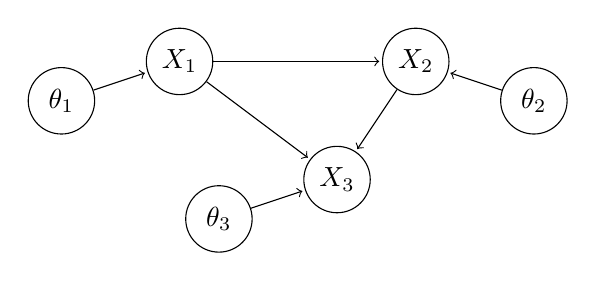
\begin{tikzpicture}[shorten >=1pt,->]
      \tikzstyle{vertex}=[draw, circle,minimum size=24pt,inner sep=0pt]
      \foreach \name/\txt/\x/\y in {x1/X_1/0/0, x2/X_2/3/0, x3/X_3/2/-1.5, t1/\theta_1/-1.5/-0.5, t2/\theta_2/4.5/-0.5, t3/\theta_3/0.5/-2}
        \node[vertex] (G-\name) at (\x,\y) {$\txt$};
    
      \foreach \from/\to in {x1/x2, x2/x3, x1/x3, t1/x1, t2/x2, t3/x3}
        \draw (G-\from) -- (G-\to);
    \end{tikzpicture}
    \caption{A graph $G'$ factorizing $(\natp,X)$. Although the graph restricted on $X$ does not encode any conditional independence, $G'$ does on the joint distribution.}
    \label{fig:joint_graph}
\end{figure}
With such a graph, the Bayesian posterior can be factorized as well
\begin{align}
    p(\natp|X) 
    &\propto  p(X|\natp) p(\natp)& \\
    & = \prod_i p(X_i | X_{G(i)};\natp_i) p(\natp_i)
    &(\indep_i \natp_i) \\
    & = \prod_i p(X_i | X_{G(i)};\natp_i) p(\natp_i\violet{|X_{G(i)}})
    &(\natp_i \indep X_{G(i)}) \\
    & = \prod_i p(X_i, \violet{\natp_i} | X_{G(i)})    &  \\
    & = \prod_i p(\natp_i| \violet{X_i}, X_{G(i)})p(X_i|X_{G(i)})    &  \\
    \implies p(\natp|X) 
    &= \prod_i p(\natp_i| \violet{X_i}, X_{G(i)}) \; .
\end{align}
In words, a consequence of the independence mechanism principle is that the posterior distribution of $\natp_i$ can be inferred solely from $X_i$ and its parents. 

\subsection{Equality of directions for 2 categorical variables}
In my paper on the analysis of causal speed, I proved the equivalence between sampling a joint distribution $\omega = p(A,B) \in \simplex_{K\times K}$ on $(A,B)\in \{1,\dots,K\}^2$ from a Dirichlet with parameter $\gamma\in \real_+^{K\times K}$ and sampling independently the marginal distribution $\mu = p(A)\in \simplex_K$ and the conditional distributions $\nu_i = p(B|A=i)\in\simplex_K$ from Dirichlets with respective parameters $\sum_{j=1}^K \gamma_{:,j} = \gamma \ones$ (matrix vector product) and $\gamma_{i,:}$
\begin{align}
    \underbrace{\Dir_{K^2}((\gamma_{i,j})_{i,j=1}^K) }_{p(\omega)}
    \equiv 
    \underbrace{\Dir_K\left( \gamma \ones \right)}_{p(\mu)} 
    \otimes \left (\bigotimes_{i=1}^K 
    \underbrace{\Dir_K((\gamma_{i,j})_j)}_{p(\nu_i)} 
    \right ) 
    \label{eq:dirichlet_factors}
\end{align}
Seeing data samples $(\cA,\cB) = (A_i,B_i)_{i=1}^n$ as one-hot encodings in $\real^K\times \real^K$, the posterior reads
\begin{align}
p(\mu|\cA) &= \Dir(\gamma\ones + \sum_i A_i)\\
p(\nu_k|\cA,\cB) &= \Dir(\gamma_{k,:} + \sum_i  A_{i,k} B_i ) \\
p(\omega | \cA,\cB) & = \Dir( \gamma + \sum_i A_i B_i^\top )  
\end{align}
where $A_i B_i^\top$ is the one hot matrix encoding of $A,B$.
These three posteriors are obtained independently of each other following rules of calculus for Dirichlet distributions. Yet they happen to define the same distribution on distributions, as we verify below with the two equalities from equation \eqref{eq:dirichlet_factors}.
\begin{align}
    \left(\gamma + \sum_i A_i B_i^\top \right)_{k,l} 
    &= \left(\gamma_{k,:} + \sum_i  A_{i,k} B_i \right)_l \\
    \left(\gamma + \sum_i A_i B_i^\top \right) \ones 
    &= \gamma \ones + \sum_i A_i \; .
\end{align}
The interpretation of this result is that \emph{taking the posterior with the decomposition $A\rightarrow B$ or $B\rightarrow A$ give the same result}. As a corollary the MAP is also the same
\begin{align}
\hat \omega^\text{MAP} 
= \frac{\gamma + \sum_i A_i B_i^\top}{\ones^\top (\gamma + \sum_i A_i B_i^\top) \ones}
=\frac{\gamma + \sum_i A_i B_i^\top}{n_0 + n}
\end{align}
Using Bayesian statistics with this prior, there is no distinction between directions.

Is this bound to happen with a symmetric prior ? Let's give a name to the change of variable $f(\omega) = \mu,\nu$. 
Remark that $f(\omega^\top) = \mu_\leftarrow, \nu_\leftarrow$, eg in the categorical special case transposing omega and changing variables give the anticausal direction. 
For sure  $p(X|\mu,\nu) = p(X|f(\omega)) = p(X|\omega)$. 
Using the change of variable formula  we get something.
But which equality am I looking for exactly ? 
\end{document}